\documentclass{beamer}
\usepackage{graphicx}
\usepackage{xcolor}
\usepackage{tikz}
\usepackage{amsmath}

% 自定义颜色
\definecolor{purpleblue}{RGB}{80, 80, 180}
\definecolor{lightgray}{RGB}{230, 230, 230}
\definecolor{novelPurple}{RGB}{98, 54, 255} 
\definecolor{darkgray}{RGB}{50, 50, 50}

% 主题设置
\usetheme{Madrid}  
\usecolortheme{dolphin} 

% 设置字体
\setbeamerfont{title}{size=\Large,series=\bfseries}
\setbeamerfont{frametitle}{size=\LARGE,series=\bfseries}
\setbeamercolor{frametitle}{fg=white, bg=novelPurple}
\setbeamercolor{title}{fg=white, bg=purpleblue}

% 封面信息
\title[SAT Unit 1.3 ]{\textbf{SAT Unit 1.3 \\Linear Equation in Two Variables}}
\author{\textbf{Jack Zeng}}
\institute{\textcolor{white}{\textbf{Novel Prep}}}
\date{\today} 

\begin{document}

% --- Title Slide ---
\begin{frame}
    \titlepage
    \vfill
    \begin{flushright}
        \textcolor{purpleblue}{\Huge \textbf{Novel Prep}}
    \end{flushright}
\end{frame}


% --- Custom Background Slide ---
\begin{frame}

    \begin{tikzpicture}[remember picture, overlay]
        % 设置浅色渐变背景
        \shade[top color=softPurple, bottom color=softGray] 
            (current page.north west) rectangle (current page.south east);
        
        % 添加高斯模糊光晕
        \fill[white, opacity=0.3] (current page.center) circle (4cm);
        
        % 主标题
        \node[align=center] at (current page.center) {
            {\Huge\bfseries\textcolor{purpleblue}{Novel Prep}} \\[0.5cm]
            {\Large\itshape\textcolor{lightText}{Excellence in SAT Prep}}
        };

        % 添加柔和光点（点缀）
        \foreach \x in {1,2,3,4,5} {
            \fill[purpleblue, opacity=0.2] (rand*10-5, rand*7-3.5) circle (0.1+\x*0.05);
        }

        ;
    \end{tikzpicture}
\end{frame}


\begin{frame}{Overview}
    \tableofcontents
\end{frame}




% --- Slide 1: Introduction ---
\begin{frame}{Introduction to Linear Equations in Two Variables}
    \textbf{Definition:}  
    A linear equation in two variables is an equation that can be written in the form:
    \[
    ax + by = c
    \]
    where:
    \begin{itemize}
        \item \( a, b, c \) are real numbers.
        \item \( x \) and \( y \) are variables.
        \item \( a \) and \( b \) are not both zero.
    \end{itemize}

    \vspace{0.5cm}
    \textbf{Example:}  
    \[
    2x + 3y = 6
    \]
    is a linear equation because it has two variables and forms a straight line when graphed.
\end{frame}
\begin{frame}
\section{Three Forms of Linear Equations}
    \begin{tikzpicture}[remember picture, overlay]
        \shade[top color=softPurple, bottom color=softGray] 
            (current page.north west) rectangle (current page.south east);
        \fill[white, opacity=0.3] (current page.center) circle (4cm);
        \node[align=center] at (current page.center) {
            {\huge\bfseries\textcolor{purpleblue}{Three Forms of Linear Equations}} \\[0.5cm]
            {\large\itshape\textcolor{lightText}{Excellence in SAT Prep}}
        };
        \foreach \x in {1,2,3,4,5} {
            \fill[purpleblue, opacity=0.2] (rand*10-5, rand*7-3.5) circle (0.1+\x*0.05);
        }
        ;
    \end{tikzpicture}
\end{frame}
% --- Slide 2: Standard Form ---
\begin{frame}{Standard Form of a Linear Equation}
    \textbf{Standard Form:}  
    \[
    Ax + By = C
    \]
    \begin{itemize}
        \item \( A, B, C \) are real numbers.
        \item \( A \) and \( B \) are not both zero.
    \end{itemize}

    \vspace{0.5cm}
    \textbf{Examples:}
    \begin{itemize}
        \item \( 5x - 2y = 10 \)
        \item \( 3x + 4y = 8 \)
        \item \( y = -2x + 7 \) (This is not in standard form, but can be rewritten as \( 2x + y = 7 \)).
    \end{itemize}
\end{frame}

\begin{frame}{\textbf{Question: Training Course Duration Difference}}
    A certain apprentice has enrolled in \textbf{85} hours of training courses. The equation
    \[
    10x + 15y = 85
    \]
    represents this situation, where \( x \) is the number of on-site training courses and \( y \) is the number of online training courses this apprentice has enrolled in.

    \vspace{0.3cm}
    How many more hours does \textbf{each} online training course take than \textbf{each} on-site training course?
\end{frame}

% --- Answer Explanation ---
\begin{frame}{\textbf{Answer Explanation: Training Course Duration Difference}}
    \textbf{Solution:}
    \begin{itemize}
        \item The coefficient of \( x \) (on-site training) is \textbf{10}, meaning each on-site training course lasts 10 hours.
        \item The coefficient of \( y \) (online training) is \textbf{15}, meaning \textbf{each} online training course lasts 15 hours.
        \item The difference in duration per course:
        \[
        15 - 10 = 5.
        \]
    \end{itemize}

    \textbf{Final Answer:} Each online training course takes \(\mathbf{5}\) more hours than each on-site training course.
\end{frame}



\begin{frame}{Understanding X-Intercept and Y-Intercept}
    \textbf{Definition:}
    \begin{itemize}
        \item The \textbf{x-intercept} is the point where the line crosses the x-axis. At this point, \( y = 0 \).
        \item The \textbf{y-intercept} is the point where the line crosses the y-axis. At this point, \( x = 0 \).
    \end{itemize}

    \vspace{0.5cm}
    \textbf{How to Find Intercepts:}
    \begin{enumerate}
        \item To find the \textbf{x-intercept}, set \( y = 0 \) in the equation and solve for \( x \).
        \item To find the \textbf{y-intercept}, set \( x = 0 \) in the equation and solve for \( y \).
    \end{enumerate}

    \vspace{0.5cm}

\end{frame}

\begin{frame}{Understanding X-Intercept and Y-Intercept}
    \textbf{Example: Given the equation \( 3x - 2y = 6 \)}
    \begin{itemize}
        \item \textbf{Find the x-intercept:} Set \( y = 0 \), solve for \( x \).
        \[
        3x - 2(0) = 6  \quad \Rightarrow \quad 3x = 6 \quad \Rightarrow \quad x = 2
        \]
        \textcolor{blue}{The x-intercept is \( (2, 0) \)}.
        
        \item \textbf{Find the y-intercept:} Set \( x = 0 \), solve for \( y \).
        \[
        3(0) - 2y = 6  \quad \Rightarrow \quad -2y = 6 \quad \Rightarrow \quad y = -3
        \]
        \textcolor{red}{The y-intercept is \( (0, -3) \)}.
    \end{itemize}
    
\end{frame}

\begin{frame}{\textbf{Question: Finding \( \frac{b}{a} \)}}
    The graph of \( 7x + 2y = -31 \) in the \( xy \)-plane has an \( x \)-intercept at \( (a, 0) \) and a \( y \)-intercept at \( (0, b) \), where \( a \) and \( b \) are constants.  

    \vspace{0.3cm}
    What is the value of \( \frac{b}{a} \)?

    \vspace{0.5cm}
    \textbf{Options:}
    \begin{enumerate}
        \item[A.] \( -\frac{7}{2} \)
        \item[B.] \( -\frac{2}{7} \)
        \item[C.] \( \frac{2}{7} \)
        \item[D.] \( \frac{7}{2} \)
    \end{enumerate}
\end{frame}

% --- Answer Explanation ---
\begin{frame}{\textbf{Answer Explanation: Finding \( \frac{b}{a} \)}}
    \textbf{Solution:}
    \begin{itemize}
        \item The \( x \)-intercept is found by setting \( y = 0 \) in the equation \( 7x + 2y = -31 \):
        \[
        7x + 2(0) = -31 \Rightarrow x = -\frac{31}{7}.
        \]
        Thus, \( a = -\frac{31}{7} \).

        \item The \( y \)-intercept is found by setting \( x = 0 \) in the equation:
        \[
        7(0) + 2y = -31 \Rightarrow y = -\frac{31}{2}.
        \]
        Thus, \( b = -\frac{31}{2} \).

        \item Compute \( \frac{b}{a} \):
        \[
        \frac{b}{a} = \frac{-\frac{31}{2}}{-\frac{31}{7}} = \frac{31}{2} \times \frac{7}{31} = \frac{7}{2}.
        \]

    \end{itemize}
    \textbf{Final Answer:} \( \boxed{\frac{7}{2}} \).
\end{frame}





\begin{frame}{Slope-Intercept Form}
    \textbf{Equation:}
    \[
    y = mx + b
    \]
    where:
    \begin{itemize}
        \item \( m \) is the slope (rate of change).
        \item \( b \) is the y-intercept (where the line crosses the y-axis).
    \end{itemize}

    \vspace{0.5cm}
    \textbf{Example:}
    \[
    y = 2x + 3
    \]
    \begin{itemize}
        \item Slope = 2 (the line rises 2 units for every 1 unit increase in \( x \)).
        \item Y-intercept = 3 (crosses the y-axis at 3).
    \end{itemize}
\end{frame}





\begin{frame}{Point-Slope Form}
    \textbf{Equation:}
    \[
    y - y_1 = m(x - x_1)
    \]
    where:
    \begin{itemize}
        \item \( (x_1, y_1) \) is a given point on the line.
        \item \( m \) is the slope.
    \end{itemize}

    \vspace{0.5cm}
    \textbf{Example:} Given a point \( (2, 5) \) and slope \( m = 3 \), the equation is:
    \[
    y - 5 = 3(x - 2)
    \]
    which can be rewritten in slope-intercept form as:
    \[
    y = 3x - 1
    \]
\end{frame}
\begin{frame}
\section{Transformation of a Linear Line}
    \begin{tikzpicture}[remember picture, overlay]
        \shade[top color=softPurple, bottom color=softGray] 
            (current page.north west) rectangle (current page.south east);
        \fill[white, opacity=0.3] (current page.center) circle (4cm);
        \node[align=center] at (current page.center) {
            {\huge\bfseries\textcolor{purpleblue}{Transformation of a Linear Line}} \\[0.5cm]
            {\large\itshape\textcolor{lightText}{Excellence in SAT Prep}}
        };
        \foreach \x in {1,2,3,4,5} {
            \fill[purpleblue, opacity=0.2] (rand*10-5, rand*7-3.5) circle (0.1+\x*0.05);
        }
        ;
    \end{tikzpicture}
\end{frame}
% --- Slide 3: Graphing Linear Equations ---
\begin{frame}{Graphing a Linear Line}
    \textbf{Graphing Steps:}
    \begin{enumerate}
        \item Rewrite the equation in slope-intercept form (\( y = mx + b \)).
        \item Identify the slope (\( m \)) and y-intercept (\( b \)).
        \item Plot the y-intercept.
        \item Use the slope to find another point.
        \item Draw a straight line through the points.
    \end{enumerate}

    \vspace{0.5cm}
    \textbf{Example:}
    \[
    2x + 3y = 6
    \]
    Convert to slope-intercept form:
    \[
    y = -\frac{2}{3}x + 2
    \]
    \begin{itemize}
        \item Slope (\( m \)) = \( -\frac{2}{3} \)
        \item Y-intercept (\( b \)) = 2
    \end{itemize}
\end{frame}


\begin{frame}{Transformation of a Linear Equation}
    \textbf{Transformations of the linear function \( y = 2x + 1 \):}

    \begin{itemize}
        \item \textbf{Vertical Shift:} \( y = 2x + 4 \) shifts the line up by 3 units.
        \item \textbf{Horizontal Shift:} \( y = 2(x - 2) + 1 \) shifts the line right by 2 units.
        \item \textbf{Reflection:} \( y = -2x + 1 \) reflects the line over the x-axis.
        \item \textbf{Change in Slope:} \( y = 4x + 1 \) steepens the line, increasing its rate of change.
    \end{itemize}


    \begin{center}
        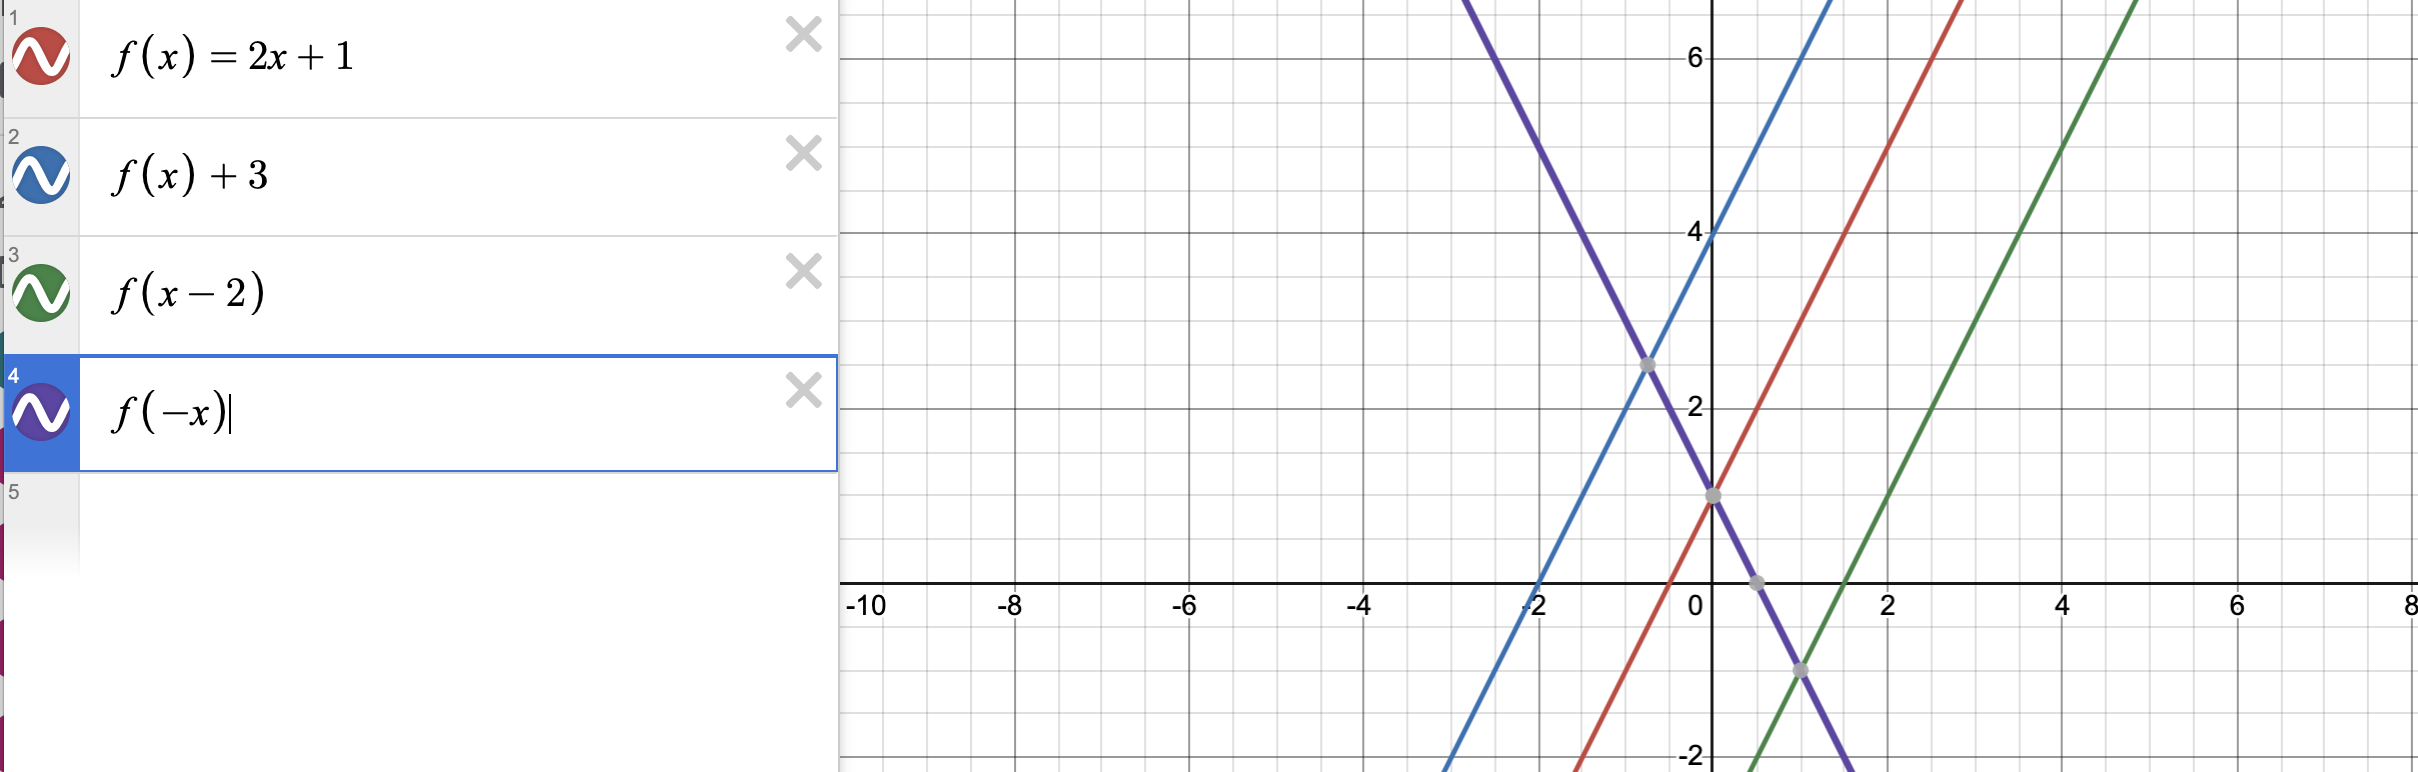
\includegraphics[width=1\linewidth]{E74.png}
    \end{center}
\end{frame}


\begin{frame}{\textbf{Question: Identifying Function \( f(x) \)}}

\begin{center}
    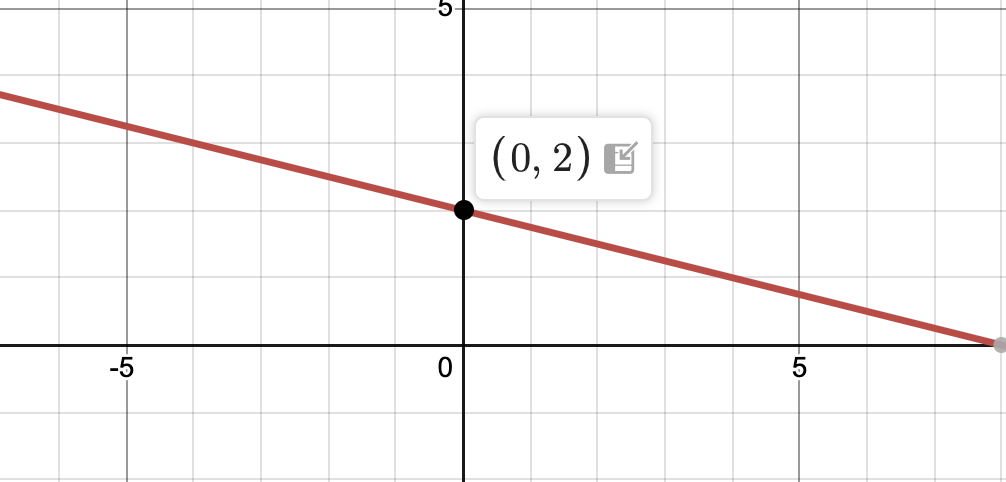
\includegraphics[width=0.5\linewidth]{E14.png}
\end{center}
    The graph of \( y = f(x) + 14 \) is shown.  

    \vspace{0.3cm}
    Which equation defines function \( f \)?

    \vspace{0.5cm}
    \textbf{Options:}
    \begin{enumerate}
        \item[A.] \( f(x) = -\frac{1}{4}x - 12 \)
        \item[B.] \( f(x) = -\frac{1}{4}x + 16 \)
        \item[C.] \( f(x) = -\frac{1}{4}x + 2 \)
        \item[D.] \( f(x) = -\frac{1}{4}x - 14 \)
    \end{enumerate}
\end{frame}

% --- Answer Explanation ---
\begin{frame}{\textbf{Answer Explanation: Identifying Function \( f(x) \)}}
    \textbf{Solution:}
    \begin{itemize}
        \item The given equation is \( y = f(x) + 14 \), so the graph represents \( f(x) \) shifted upward by 14 units.
        \item Identify the equation of the given graph:  
        \[
        y = -\frac{1}{4}x + 2.
        \]
        \item Since \( y = f(x) + 14 \), we solve for \( f(x) \):
        \[
        f(x) = y - 14 = -\frac{1}{4}x + 2 - 14 = -\frac{1}{4}x - 12.
        \]
    \end{itemize}

    \textbf{Final Answer:} \( \boxed{A} \).
\end{frame}

\begin{frame}
\section{Special Lines}
    \begin{tikzpicture}[remember picture, overlay]
        \shade[top color=softPurple, bottom color=softGray] 
            (current page.north west) rectangle (current page.south east);
        \fill[white, opacity=0.3] (current page.center) circle (4cm);
        \node[align=center] at (current page.center) {
            {\huge\bfseries\textcolor{purpleblue}{Special Lines}} \\[0.5cm]
            {\large\itshape\textcolor{lightText}{Excellence in SAT Prep}}
        };
        \foreach \x in {1,2,3,4,5} {
            \fill[purpleblue, opacity=0.2] (rand*10-5, rand*7-3.5) circle (0.1+\x*0.05);
        }
        ;
    \end{tikzpicture}
\end{frame}
\begin{frame}{Parallel and Perpendicular Line Theorems}
    \textbf{Parallel Line Theorem:}
    \begin{itemize}
        \item Two non-vertical lines are \textbf{parallel} if and only if they have the \textbf{same slope}.
        \item Mathematically, if two lines have equations:
        \[
        y = m_1x + b_1 \quad \text{and} \quad y = m_2x + b_2
        \]
        then the lines are parallel if:
        \[
        m_1 = m_2
        \]
    \end{itemize}

\pause
    \vspace{0.5cm}
    \textbf{Perpendicular Line Theorem:}
    \begin{itemize}
        \item Two non-vertical lines are \textbf{perpendicular} if and only if the product of their slopes is \(-1\).
        \item Mathematically, if two lines have slopes \( m_1 \) and \( m_2 \), then they are perpendicular if:
        \[
        m_1 \cdot m_2 = -1
        \]
    \end{itemize}

    \vspace{0.5cm}
    \textbf{Example:}
    \begin{itemize}
        \item The lines \( y = 2x + 3 \) and \( y = 2x - 5 \) are parallel because their slopes are both \( 2 \).
        \item The lines \( y = \frac{3}{4}x + 1 \) and \( y = -\frac{4}{3}x - 2 \) are perpendicular because:
        \[
        \left(\frac{3}{4} \right) \times \left(-\frac{4}{3} \right) = -1
        \]
    \end{itemize}
\end{frame}

\begin{frame}{\textbf{Question: Finding the Value of \( d \)}}
    In the \( xy \)-plane, line \( \ell \) passes through the point \( (0,0) \) and is parallel to the line represented by the equation:
    \[
    y = 8x + 2.
    \]
    If line \( \ell \) also passes through the point \( (3,d) \), what is the value of \( d \)?
\end{frame}

% --- Answer Explanation ---
\begin{frame}{\textbf{Answer Explanation: Finding the Value of \( d \)}}
    \textbf{Solution:}
    \begin{itemize}
        \item Since line \( \ell \) is parallel to \( y = 8x + 2 \), it has the same slope \( m = 8 \).
        \item The equation of line \( \ell \), passing through \( (0,0) \), is:
        \[
        y = 8x.
        \]
        \item Substitute \( x = 3 \) to find \( d \):
        \[
        d = 8(3) = 24.
        \]
    \end{itemize}
    \textbf{Final Answer:} \( \boxed{24} \).
\end{frame}

\begin{frame}{\textbf{Question: Finding the Slope of Line \( r \)}}
    Line \( p \) is defined by the equation:
    \[
    4y + 8x = 6.
    \]
    Line \( r \) is perpendicular to line \( p \) in the \( xy \)-plane.  
    What is the slope of line \( r \)?
\end{frame}

% --- Answer Explanation ---
\begin{frame}{\textbf{Answer Explanation: Finding the Slope of Line \( r \)}}
    \textbf{Solution:}
    \begin{itemize}
        \item Rewrite the equation of line \( p \) in slope-intercept form:
        \[
        4y = -8x + 6.
        \]
        \[
        y = -2x + \frac{3}{2}.
        \]
        \item The slope of line \( p \) is \( m_p = -2 \).
        \item Since line \( r \) is perpendicular to line \( p \), its slope is the negative reciprocal of \( -2 \):
        \[
        m_r = \frac{1}{2}.
        \]
    \end{itemize}
    \textbf{Final Answer:} \( \boxed{\frac{1}{2}} \).
\end{frame}




\begin{frame}
    \begin{tikzpicture}[remember picture, overlay]
        \shade[top color=softPurple, bottom color=softGray] 
            (current page.north west) rectangle (current page.south east);
        \fill[white, opacity=0.3] (current page.center) circle (4cm);
        \node[align=center] at (current page.center) {
            {\huge\bfseries\textcolor{purpleblue}{Real World Application}} \\[0.5cm]
            {\large\itshape\textcolor{lightText}{Excellence in SAT Prep}}
        };
        \foreach \x in {1,2,3,4,5} {
            \fill[purpleblue, opacity=0.2] (rand*10-5, rand*7-3.5) circle (0.1+\x*0.05);
        }
        ;
    \end{tikzpicture}
\end{frame}


% --- Slide 5: Applications in Real Life ---
\begin{frame}{Real-World Applications}
\section{Real World Application}
    Linear equations in two variables appear in various real-life scenarios:

    \begin{itemize}
        \item \textbf{Business:} Predicting profit and expenses.
        \item \textbf{Physics:} Calculating velocity and motion.
        \item \textbf{Economics:} Supply and demand relationships.
        \item \textbf{Engineering:} Designing bridges and buildings.
    \end{itemize}

    \vspace{0.5cm}
    \textbf{Example:}  
    A company’s total cost equation is:
    \[
    C = 50x + 200
    \]
    where:
    \begin{itemize}
        \item \( C \) is the total cost.
        \item \( x \) is the number of products made.
        \item \( 50 \) is the cost per product.
        \item \( 200 \) is the fixed cost.
    \end{itemize}
\end{frame}


\begin{frame}{\textbf{Question: Mixing Saline Solutions}}
    How many liters of a 25\% saline solution must be added to 3 liters of a 10\% saline solution to obtain a 15\% saline solution?


\end{frame}

\begin{frame}{Solution}
    \textbf{Solution:}
    \begin{itemize}
        \item Let \( x \) be the amount of 25\% saline solution to be added.
        \item The total salt in the solutions:
        \[
        0.10(3) + 0.25(x) = 0.15(3 + x).
        \]
        \item Solve for \( x \):
        \[
        0.3 + 0.25x = 0.45 + 0.15x.
        \]
        \[
        0.25x - 0.15x = 0.45 - 0.3.
        \]
        \[
        0.10x = 0.15.
        \]
        \[
        x = 1.5.
        \]
    \end{itemize}
    \textbf{Final Answer:} \(\boxed{1.5}\) liters.
    
\end{frame}

\begin{frame}
    \begin{tikzpicture}[remember picture, overlay]
        \shade[top color=softPurple, bottom color=softGray] 
            (current page.north west) rectangle (current page.south east);
        \fill[white, opacity=0.3] (current page.center) circle (4cm);
        \node[align=center] at (current page.center) {
            {\huge\bfseries\textcolor{purpleblue}{Practices}} \\[0.5cm]
            {\large\itshape\textcolor{lightText}{Excellence in SAT Prep}}
        };
        \foreach \x in {1,2,3,4,5} {
            \fill[purpleblue, opacity=0.2] (rand*10-5, rand*7-3.5) circle (0.1+\x*0.05);
        }
        ;
    \end{tikzpicture}
\end{frame}

\begin{frame}{Question: Sticker Sheet Interpretation}
A teacher printed sticker sheets with 7 stickers on each sheet. At a school party, she gave out 2 stickers to each student who attended. The relationship between the number of students who attended the party, \(x\), and the number of sticker sheets that the teacher printed, \(y\), is represented by the equation:
\[
7y - 32 = 2x
\]
What is the best interpretation of the number \(32\) in this context?

\vspace{1em}
\begin{itemize}
    \item[\textbf{A.}] The teacher gave out a total of 32 stickers at the party.
    \item[\textbf{B.}] The teacher had 32 sticker sheets remaining after the party.
    \item[\textbf{C.}] The teacher printed 32 more stickers than she gave out at the party.
    \item[\textbf{D.}] The teacher printed a total of 32 sticker sheets.
\end{itemize}
\end{frame}
\begin{frame}{Answer: Sticker Sheet Interpretation}
We are given:
\[
7y - 32 = 2x
\]
Here, \(7y\) represents the total number of stickers printed (7 stickers per sheet × \(y\) sheets),  
and \(2x\) represents the total number of stickers given out (2 stickers per student × \(x\) students).

So, \(7y - 32 = 2x\) means the teacher gave out 32 fewer stickers than she printed.

\vspace{1em}
\textbf{Correct Interpretation:}  
\textbf{C.} The teacher printed 32 more stickers than she gave out at the party.
\end{frame}

\begin{frame}{Question: Perpendicular Line}
Line \( m \) passes through the point \( (-2, 4) \) and is \textbf{perpendicular} to the line:
\[
y = \frac{1}{2}x - 3
\]
Which of the following is the equation of line \( m \)?
\begin{itemize}
    \item[\textbf{A.}] \( y = -2x \)
    \item[\textbf{B.}] \( y = -2x + 4 \)
    \item[\textbf{C.}] \( y = 2x + 8 \)
    \item[\textbf{D.}] \( y = -2x + 2 \)
\end{itemize}
\end{frame}


\begin{frame}{Answer: Perpendicular Line}
The original slope is \( \frac{1}{2} \), so the perpendicular slope is the \textbf{negative reciprocal}:
\[
m = -2
\]

Use point-slope form with point \( (-2, 4) \):
\[
y - 4 = -2(x + 2) \Rightarrow y = -2x - 4 + 4 = -2x
\Rightarrow \boxed{\text{A. } y = -2x}
\]
\end{frame}


\begin{frame}{Challenge: Relationship Between Two Lines}
Lines \( L_1 \) and \( L_2 \) have the following equations:

\[
L_1: 3x + 4y = 12 
\]
\[
L_2: 4x - 3y = 5\]

Which of the following best describes the relationship between \( L_1 \) and \( L_2 \)?
\begin{itemize}
    \item[\textbf{A.}] The lines are parallel.
    \item[\textbf{B.}] The lines are perpendicular.
    \item[\textbf{C.}] The lines intersect but are neither perpendicular nor parallel.
    \item[\textbf{D.}] The lines are identical.
\end{itemize}
\end{frame}

\begin{frame}{Answer: Line Relationship}
Convert both to slope-intercept form:

\textbf{Line 1:}
\[
3x + 4y = 12 \Rightarrow 4y = -3x + 12 \Rightarrow y = -\frac{3}{4}x + 3
\]

\textbf{Line 2:}
\[
4x - 3y = 5 \Rightarrow -3y = -4x + 5 \Rightarrow y = \frac{4}{3}x - \frac{5}{3}
\]

Slopes: \( m_1 = -\frac{3}{4}, m_2 = \frac{4}{3} \Rightarrow m_1 \cdot m_2 = -1 \)

\textbf{Result: The lines are perpendicular.}

\[
\boxed{\text{Correct Answer: B.}}
\]
\end{frame}



\begin{frame}{Question}

\vspace{1em}

The table below shows the coordinates of three points on a line in the $xy$-plane, where $k$ and $n$ are constants. If the slope of the line is $2$, what is the value of $k + n$?

\vspace{1em}

\[
\begin{array}{c|c}
x & y \\
\hline
3 & 7 \\
k & 11 \\
12 & n \\
\end{array}
\]

\end{frame}


\begin{frame}{Answer}
\footnotesize
\textbf{Step 1.} The slope of the line is $2$, so:

\[
\text{slope} = \frac{y_2 - y_1}{x_2 - x_1} = 2
\]

\vspace{0.5em}
\textbf{Step 2.} Use points $(3,7)$ and $(k,11)$:

\[
2 = \frac{11 - 7}{k - 3}
\]

\[
k = 5
\]

\vspace{0.5em}
\textbf{Step 3.} Use points $(3,7)$ and $(12,n)$:

\[
2 = \frac{n - 7}{12 - 3}
\]

\[
n = 25
\]

\vspace{0.5em}
\textbf{Step 4.} Then:

\[
k + n = 5 + 25 = \boxed{30}
\]

\end{frame}


\begin{frame}{\textbf{Question: Identifying Perpendicular Line Pairs}}
    \small
    Consider the given system of equations:
    \[
    5x + 7y = 1
    \]
    \[
    ax + by = 1
    \]
    where \( a \) and \( b \) are constants. The graph of these equations represents a pair of perpendicular lines.

    \vspace{0.3cm}
    Which of the following systems also represents a pair of perpendicular lines?

    \vspace{0.4cm}
    \textbf{Options:}
    \begin{itemize}
        \item \textbf{A:} \( 10x + 7y = 1 \), \quad \( ax - 2by = 1 \)
        \item \textbf{B:} \( 10x + 7y = 1 \), \quad \( ax + 2by = 1 \)
        \item \textbf{C:} \( 10x + 7y = 1 \), \quad \( 2ax + by = 1 \)
        \item \textbf{D:} \( 5x - 7y = 1 \), \quad \( ax + by = 1 \)
    \end{itemize}
\end{frame}


% --- Answer Explanation ---
\begin{frame}{\textbf{Answer Explanation: Identifying Perpendicular Line Pairs}}
    \textbf{Correct Answer: \textcolor{novelPurple}{B}}  

    \vspace{0.3cm}
    \textbf{Solution:}
    \begin{itemize}
        \item Find the slope of the first equation by rewriting it in slope-intercept form:
        \[
        5x + 7y = 1 \implies y = -\frac{5}{7}x + \frac{1}{7}.
        \]
        The slope is \( -\frac{5}{7} \).
        
        \item Since the lines are perpendicular, the second equation should have a slope that is the negative reciprocal of \( -\frac{5}{7} \), which is \( \frac{7}{5} \).

        \item Checking the options, the correct system with perpendicular slopes is:
        \[
        10x + 7y = 1, \quad ax + 2by = 1.
        \]
        This corresponds to:
        \[
        \boxed{B.}
        \]
    \end{itemize}
\end{frame}






% --- Slide 7: Summary ---
\begin{frame}{Summary}
    \begin{itemize}
        \item A linear equation in two variables is written as \( Ax + By = C \).
        \item The slope (\( m \)) determines the steepness of the line.
        \item Graphing requires finding intercepts or using the slope-intercept form.
        \item Systems of linear equations can have one solution, no solution, or infinitely many solutions.
    \end{itemize}
\end{frame}


\begin{frame}{}
    \begin{tikzpicture}[remember picture, overlay]
        % 背景渐变色：蓝紫到白
        \shade[top color=novelPurple!40, bottom color=white]
            (current page.north west) rectangle (current page.south east);

        % 中心柔光
        \fill[white, opacity=0.15] (current page.center) circle (5cm);

        % 柔和光点点缀
        \foreach \x in {1,2,3,4,5} {
            \fill[novelPurple, opacity=0.12] (rand*10-5, rand*7-3.5) circle (0.1+\x*0.05);
        }
    \end{tikzpicture}

    \centering
    \vspace{5em}

    {\Huge \textbf{\textcolor{novelPurple}{Thank You!}}} \\[1em]
    {\large \textcolor{gray}{We appreciate your time and focus.}} \\[3em]

    {\LARGE \textbf{\textcolor{novelPurple}{\textsf{Novel Prep}}}}

    \vfill
\end{frame}

\end{document}
